\documentclass[12pt, titlepage, oneside]{article}
\usepackage[letterpaper, margin=1in]{geometry}
\usepackage{siunitx, booktabs, amsmath, enumitem, pdfpages, tabularx,caption, graphicx, pgfplots, textcomp}
\usepackage[siunitx]{circuitikz}
\sisetup{detect-weight=true, detect-family=true}
\usepackage{wrapfig}
\usepackage{mathrsfs}
\setlength\parindent{0pt}
\let\oldhat\hat
\let\oldvec\vec
\newcommand{\cross}{\bm{\times}}
\renewcommand{\hat}[1]{\oldhat{\mathbf{#1}}}
\usepackage{bm}
\renewcommand{\vec}[1]{\oldvec{\bm{#1}}}
\renewcommand{\hat}[1]{\oldhat{\bm{#1}}}
\renewcommand{\b}[1]{\textbf{#1}}

\begin{document}
\section*{27.1 Electric Current}
\noindent\fbox{%
	\parbox{\textwidth}{%
	\textbf{Current} is described as the amount of charge that flows through a surface. 	
	\begin{align}
	I_{avg} &= \frac{\Delta Q}{\Delta t}\\[12pt]
	I &\equiv \frac{dQ}{dt}
	\end{align}	
	1A = 1C/s
}}
\\

\noindent
The charges passing through a surface can be positive or negative, or both. The current is the amount of positive and negative charges over time.
\\
	
A charge (positive or negative) is referred to as a \textbf{charge carrier}.

\vspace{0.5cm}
\begin{wrapfigure}{r}{0.4\textwidth}
	\begin{center}\vspace{-1.1cm}
		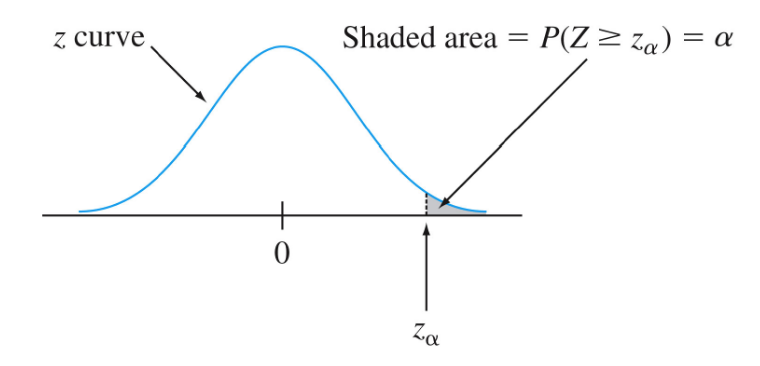
\includegraphics[scale=0.7]{1.png}
	\end{center}
\end{wrapfigure}
Consider a conductor with a cross sectional area $A$, with a length $\Delta x$. Given the charge density per unit volume is $n$. We know $q$ is the unit for one charge of the conductor. We know the volume is going to be $A \Delta x$, therefore using charge density and the unit of charge, we can derive an expression for the total charge $\Delta Q$ in this segment.
\begin{align*}
\Delta Q = (nA\Delta x)q
\end{align*}
Since we know, $\Delta x = v_d \Delta t$, we can rewrite the expression as,
\begin{align*}
\Delta Q = (nAv_d\Delta t)q
\end{align*}
Divide both sides of the equation by $\Delta t$, we are able to find the average current in the conductor,\\

\noindent\fbox{%
	\parbox{\textwidth}{%
\begin{align}
I_{avg} = \frac{\Delta Q}{\Delta t} = nqv_dA 
\end{align}
}}\\


To go back a couple of steps, $\vec{v}_d$ is known as the drift velocity. Its how the charges move on average through a conductor. When there is no field, the drift velocity is near zero. When there is a potential difference applied, the carriers will then tend their drift velocity towards a certain direction.

\newpage	
\begin{center}
		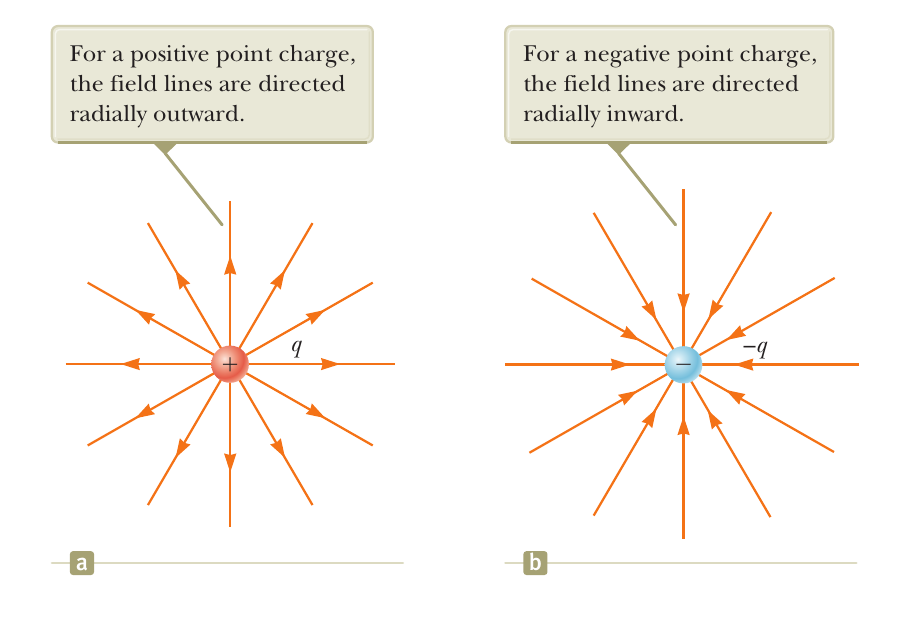
\includegraphics[scale=.7]{2.png} \hspace{2cm}
		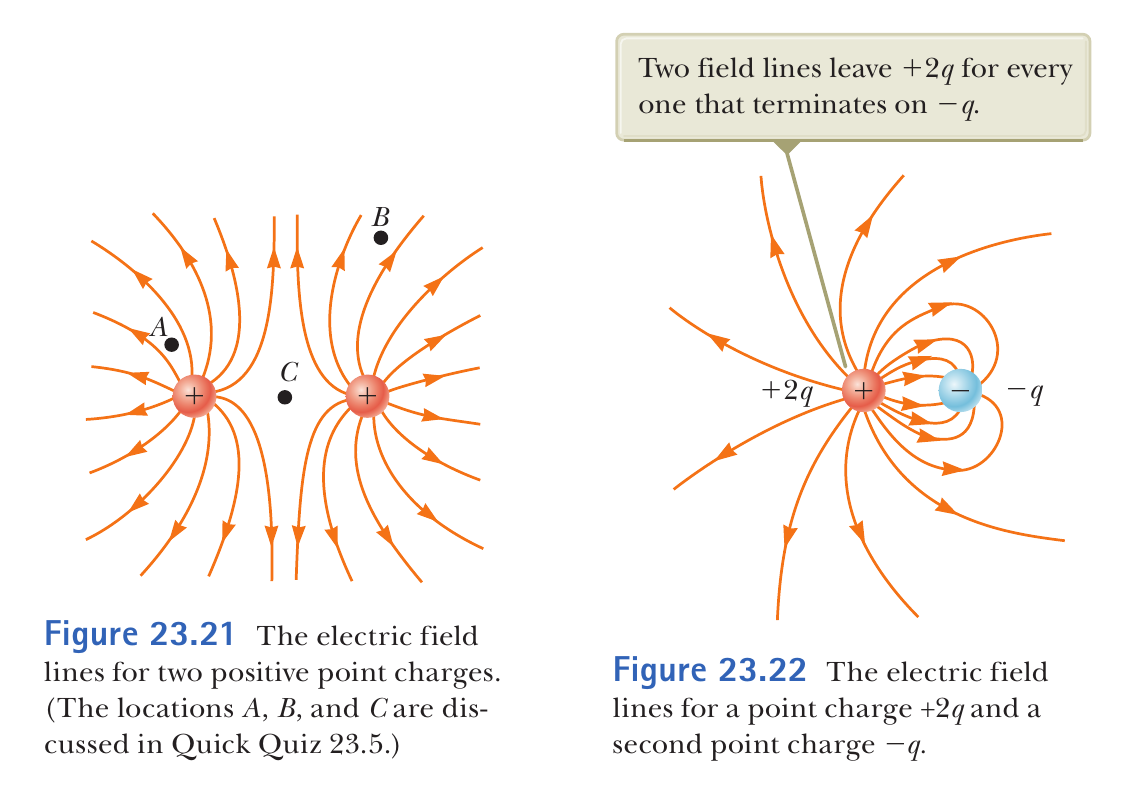
\includegraphics[scale=.7]{3.png}
\end{center}
Before and after an electric field has been applied to the conductor and how the drift velocity changes. Notice there is still bouncy and rigid movements. This is because the electrons constantly hit other atoms and their direction of their velocity varies, but notice that on average, the figure on the right has a general direction which the electrons tend towards.
\section*{27.2 Resistance}
\noindent\fbox{%
	\parbox{\textwidth}{%
		\textbf{Current Density} $J$ in the conductor is defined as the current per unit area.
		\begin{align}
		J \equiv \frac{I}{A} = nqv_d
		\end{align}	
		For some conductor of cross sectional area $A$ carrying a current $I$, where $I = nqv_dA$. $[J] = \si{A/m^2}$
	}}
\\
\vspace{10pt}

\noindent\fbox{%
	\parbox{\textwidth}{%
		\textbf{Ohm's Law Condition}\\
		In some materials, the current density $J$ is proportional to the electric field $E$
		\begin{align}
		J = \sigma E
		\end{align}
		Where $\sigma$ is independent of the electric field producing the current 
	}} 
\\

Materials that have $J \propto E$ are considered to be ohmic materials (resistors). Materials that do not have this property are said to be non-ohmic (diodes). It should be noted that ohms law is not a fundamental law of nature, rather an empirical realtionship only valid for certain situations
\newpage 

\begin{wrapfigure}{r}{0.4\textwidth}
	\begin{center}\vspace{-1.1cm}
		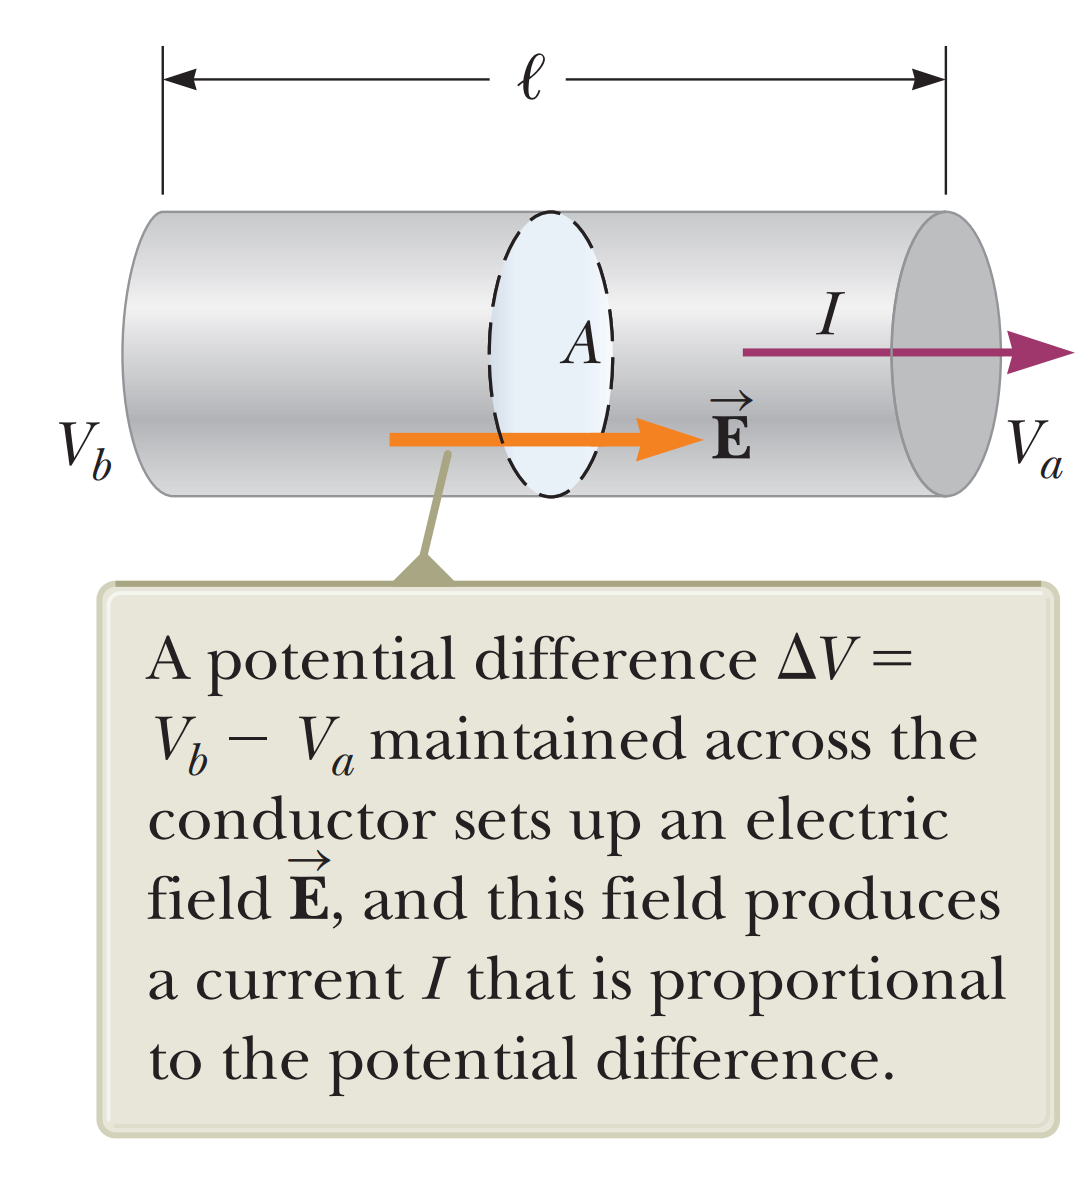
\includegraphics[scale=0.4]{4.png}
	\end{center}
\end{wrapfigure}
Consider a conductor with a cross sectional area $A$ with length $l$ with a potential difference across. We can use an equation from capter 25,
\begin{align*}
\Delta V = E l
\end{align*}
Therefore, we can express the current density $J$ in the wire as,
\begin{equation*}
J = \sigma \frac{\Delta V}{l}
\end{equation*}
Since $J = I/A$, the potential difference across the wire is,
\begin{align*}
\Delta V = \frac{l}{\sigma}J = \Bigg(\frac{l}{\sigma A}\Bigg)I = R I 
\end{align*}

\noindent\fbox{%
	\parbox{\textwidth}{%
		\textbf{Resistance}
		\begin{align}
		R \equiv \frac{\Delta V}{I}
		\end{align}
		Note: this is not ohm's law. This is the definition of resistance and is \textbf{always true}.\\
		1 \si{\ohm} $\equiv$ 1V/A
}}
\\

Ohm's law is the the linearity of $\Delta V$ and $I$. If $E$ is not linearly proportional to $J$, then $I$ vs $V$ is not linear. This would be a situation where $\sigma$, the conductivity is a function of other variables.
\\

\noindent\fbox{%
	\parbox{\textwidth}{%
		\textbf{Resistivity}
		\begin{align}
		\rho = \frac{1}{\sigma} 
		\end{align}
		$[\rho] = \si{\ohm m}$
	}}
\\

Since we know that,
\begin{align*}
R = \frac{l}{\sigma A}
\end{align*}
We can express the resistance of a uniform block of material along $l$ as,
\begin{align*}
R = \rho \frac{l}{A}
\end{align*}

Every ohmic material has a characteristic resistivity that depends on the properties of the material and on temperature. From the equation above you can see how shape of the object would change the area and therefore the resistance.\newpage

\section*{27.6 Electrical Power }
Power is the change in energy,
\begin{align*}
\frac{dU}{dt} = \frac{d}{dt}(Q\Delta V) = \frac{dQ}{dt}\Delta V = I \Delta V
\end{align*}
Note that voltage does not change over time, therefore it is a constant.
\begin{align*}
P = RI^2 = \frac{(\Delta V)^2}{R}
\end{align*}
\end{document}